\documentclass[12pt, times, a4paper]{article}

\usepackage{graphicx}

\begin{document}

\title{Kubernetes resource}
\author{Meng Oon Lee}
\date{\today}

\maketitle

\section{Kubeconfig}

\begin{enumerate}
\item Inspect the endpoints for the cluster and installed add-ons. \\
\textbf{kubectl cluster-info} \\
\newline
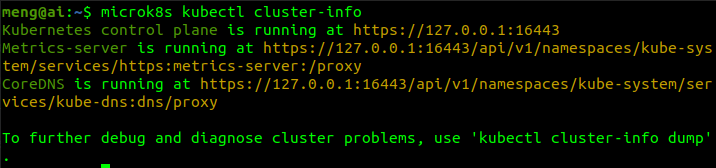
\includegraphics[width=\textwidth]{fig/Kubeconfig/cluster-info.png}
\item List all the nodes in the cluster. To get a more detailed view of the nodes, the `-o wide` flag can be passed. \\
\textbf{kubectl get nodes [-o wide]} \\
\newline
\item Describe a cluster node. Typical configuration: node IP. \\
\textbf{kubectl describe node \{NODE\}}
\newline
\end{enumerate}

\end{document}
